\documentclass[twoside]{article}
%\usepackage{graphicx}
%\usepackage{caption}
\usepackage{subcaption}
\usepackage[letterpaper, margin=1in]{geometry}
\usepackage{float}
\usepackage{fancyhdr}
\usepackage{tikz}
\usepackage[utf8]{inputenc}
\usepackage{ifthen}
\usepackage{tabu}
\usepackage[shortlabels]{enumitem}
\usepackage{amsmath}
\usetikzlibrary{fadings}



\pagestyle{fancy}
\fancyhead{}
\fancyhead[L]{\ifthenelse{\isodd{\value{page}}}{APS Logbook}{\textbf{\rightmark}}}
\fancyhead[R]{\ifthenelse{\isodd{\value{page}}}{\textbf{\rightmark}}{Election 2016}}
\renewcommand{\headrulewidth}{1pt}
\fancyfoot{}
\fancyfoot[L]{\ifthenelse{\isodd{\value{page}}}{}{Page \thepage}}
\fancyfoot[R]{\ifthenelse{\isodd{\value{page}}}{Page \thepage}{}}



\title{American Political Systems Logbook}
\author{Noah Stockwell}
\date{2016}

\begin{document}
\begin{titlepage}
  \centering
  \begin{tikzpicture}[overlay]
  \path (0,0) rectangle (\paperwidth,\paperheight);
  \node[scope fading=west,inner sep=0pt,outer sep=0pt,anchor=north east,opacity=0.3] at(20,3) {
\includegraphics[height=1.0625\paperheight]{images/frontpage/flag.jpg}};
  \end{tikzpicture}
  \centering
  \begin{figure}[H]
    \centering
    \begin{subfigure}{.4\textwidth}
      \centering
      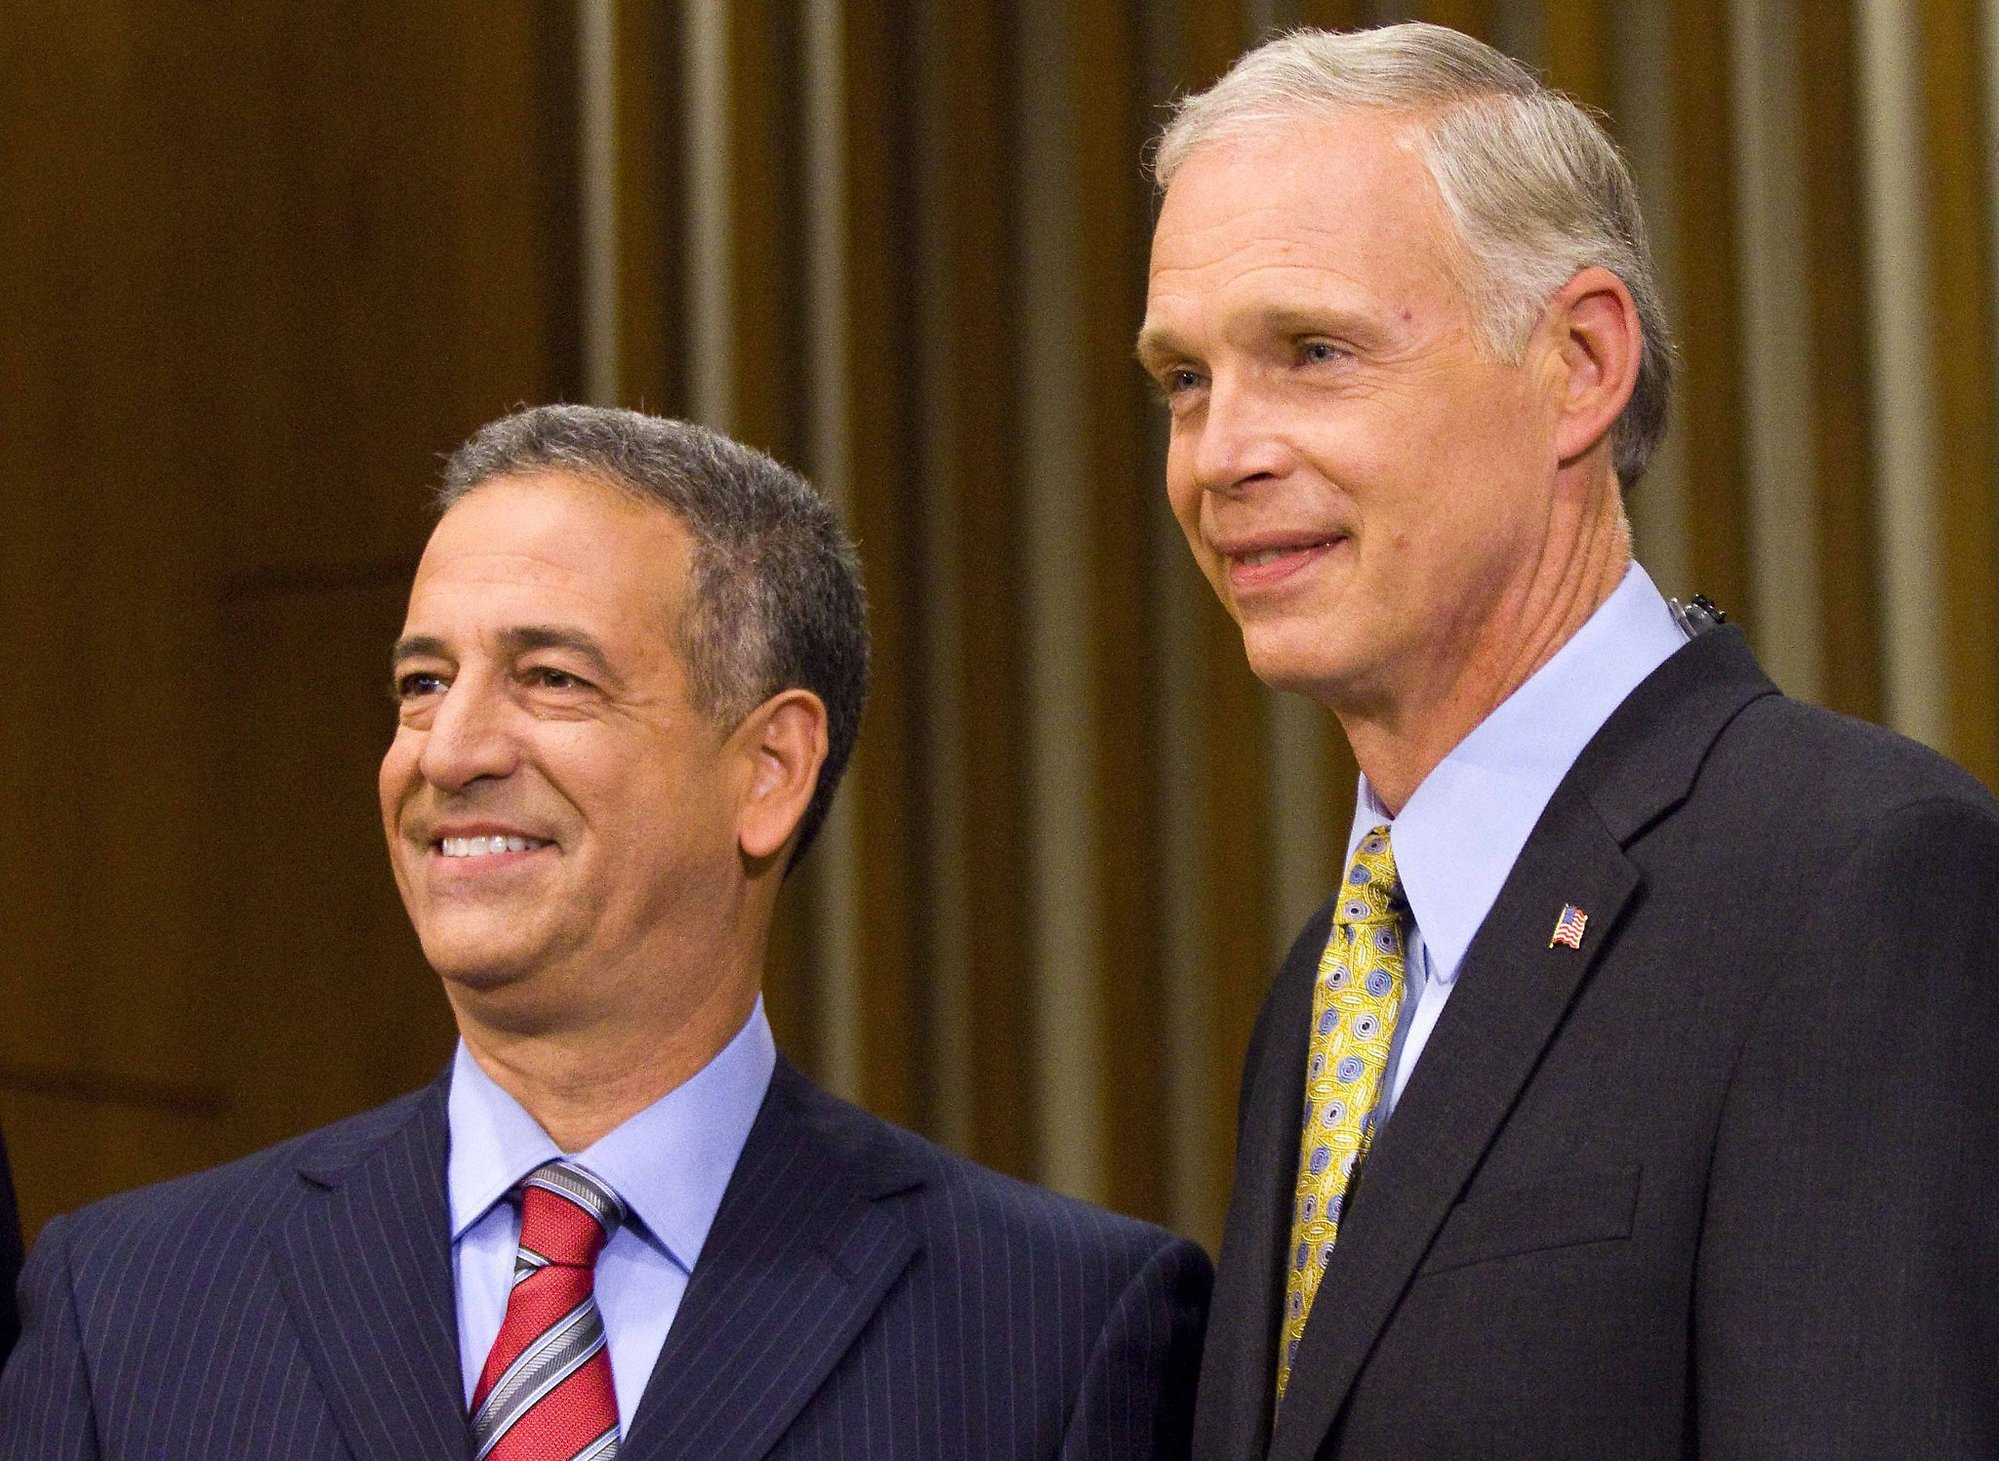
\includegraphics[width=6cm,height=4.5cm]{images/frontpage/Senate.jpg}
      \end{subfigure}%
      \begin{subfigure}{.4\textwidth}
        \centering
        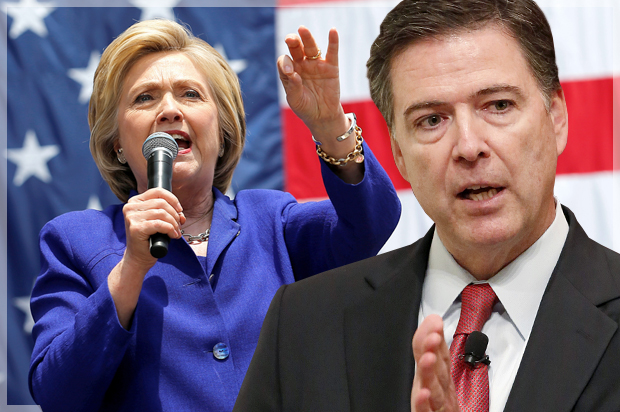
\includegraphics[width=6cm,height=4.5cm]{images/frontpage/Comey.jpg}
      \end{subfigure}%
      \centering
      \vskip3cm
    \end{figure}
    {\bfseries\huge American Political Systems Logbook\\}
    \vskip1cm
    {\bfseries\LARGE Election 2016\\}
    \vskip2cm
    {\huge Noah Stockwell\\}

    \centering
    \vskip2cm
    \centering
    \begin{figure}[H]
      \centering
      \begin{subfigure}{.4\textwidth}
        \centering
        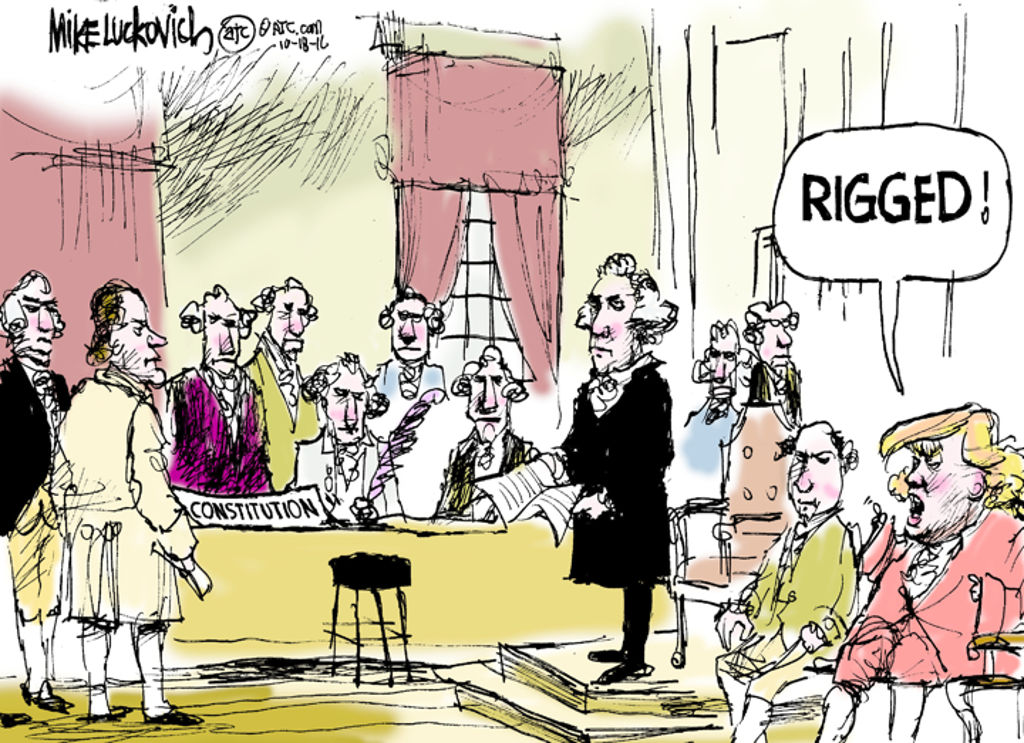
\includegraphics[width=6cm,height=4.5cm]{images/frontpage/Rigged.jpg}
        \end{subfigure}%
        \begin{subfigure}{.4\textwidth}
          \centering
          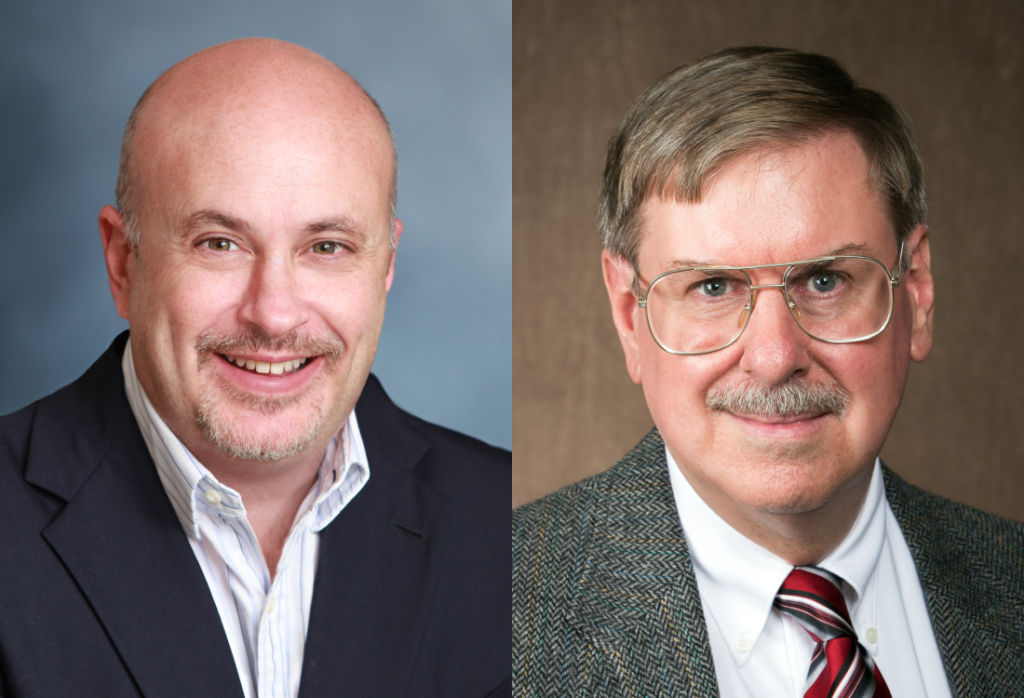
\includegraphics[width=6cm,height=4.5cm]{images/frontpage/House.jpg}
        \end{subfigure}%
      \end{figure}
\end{titlepage}
\tableofcontents
\newpage
\section{Candidate Bios}
\vskip1cm
\begin{center}
\begin{tabu} to 0.8\textwidth { X[c] X[c]}
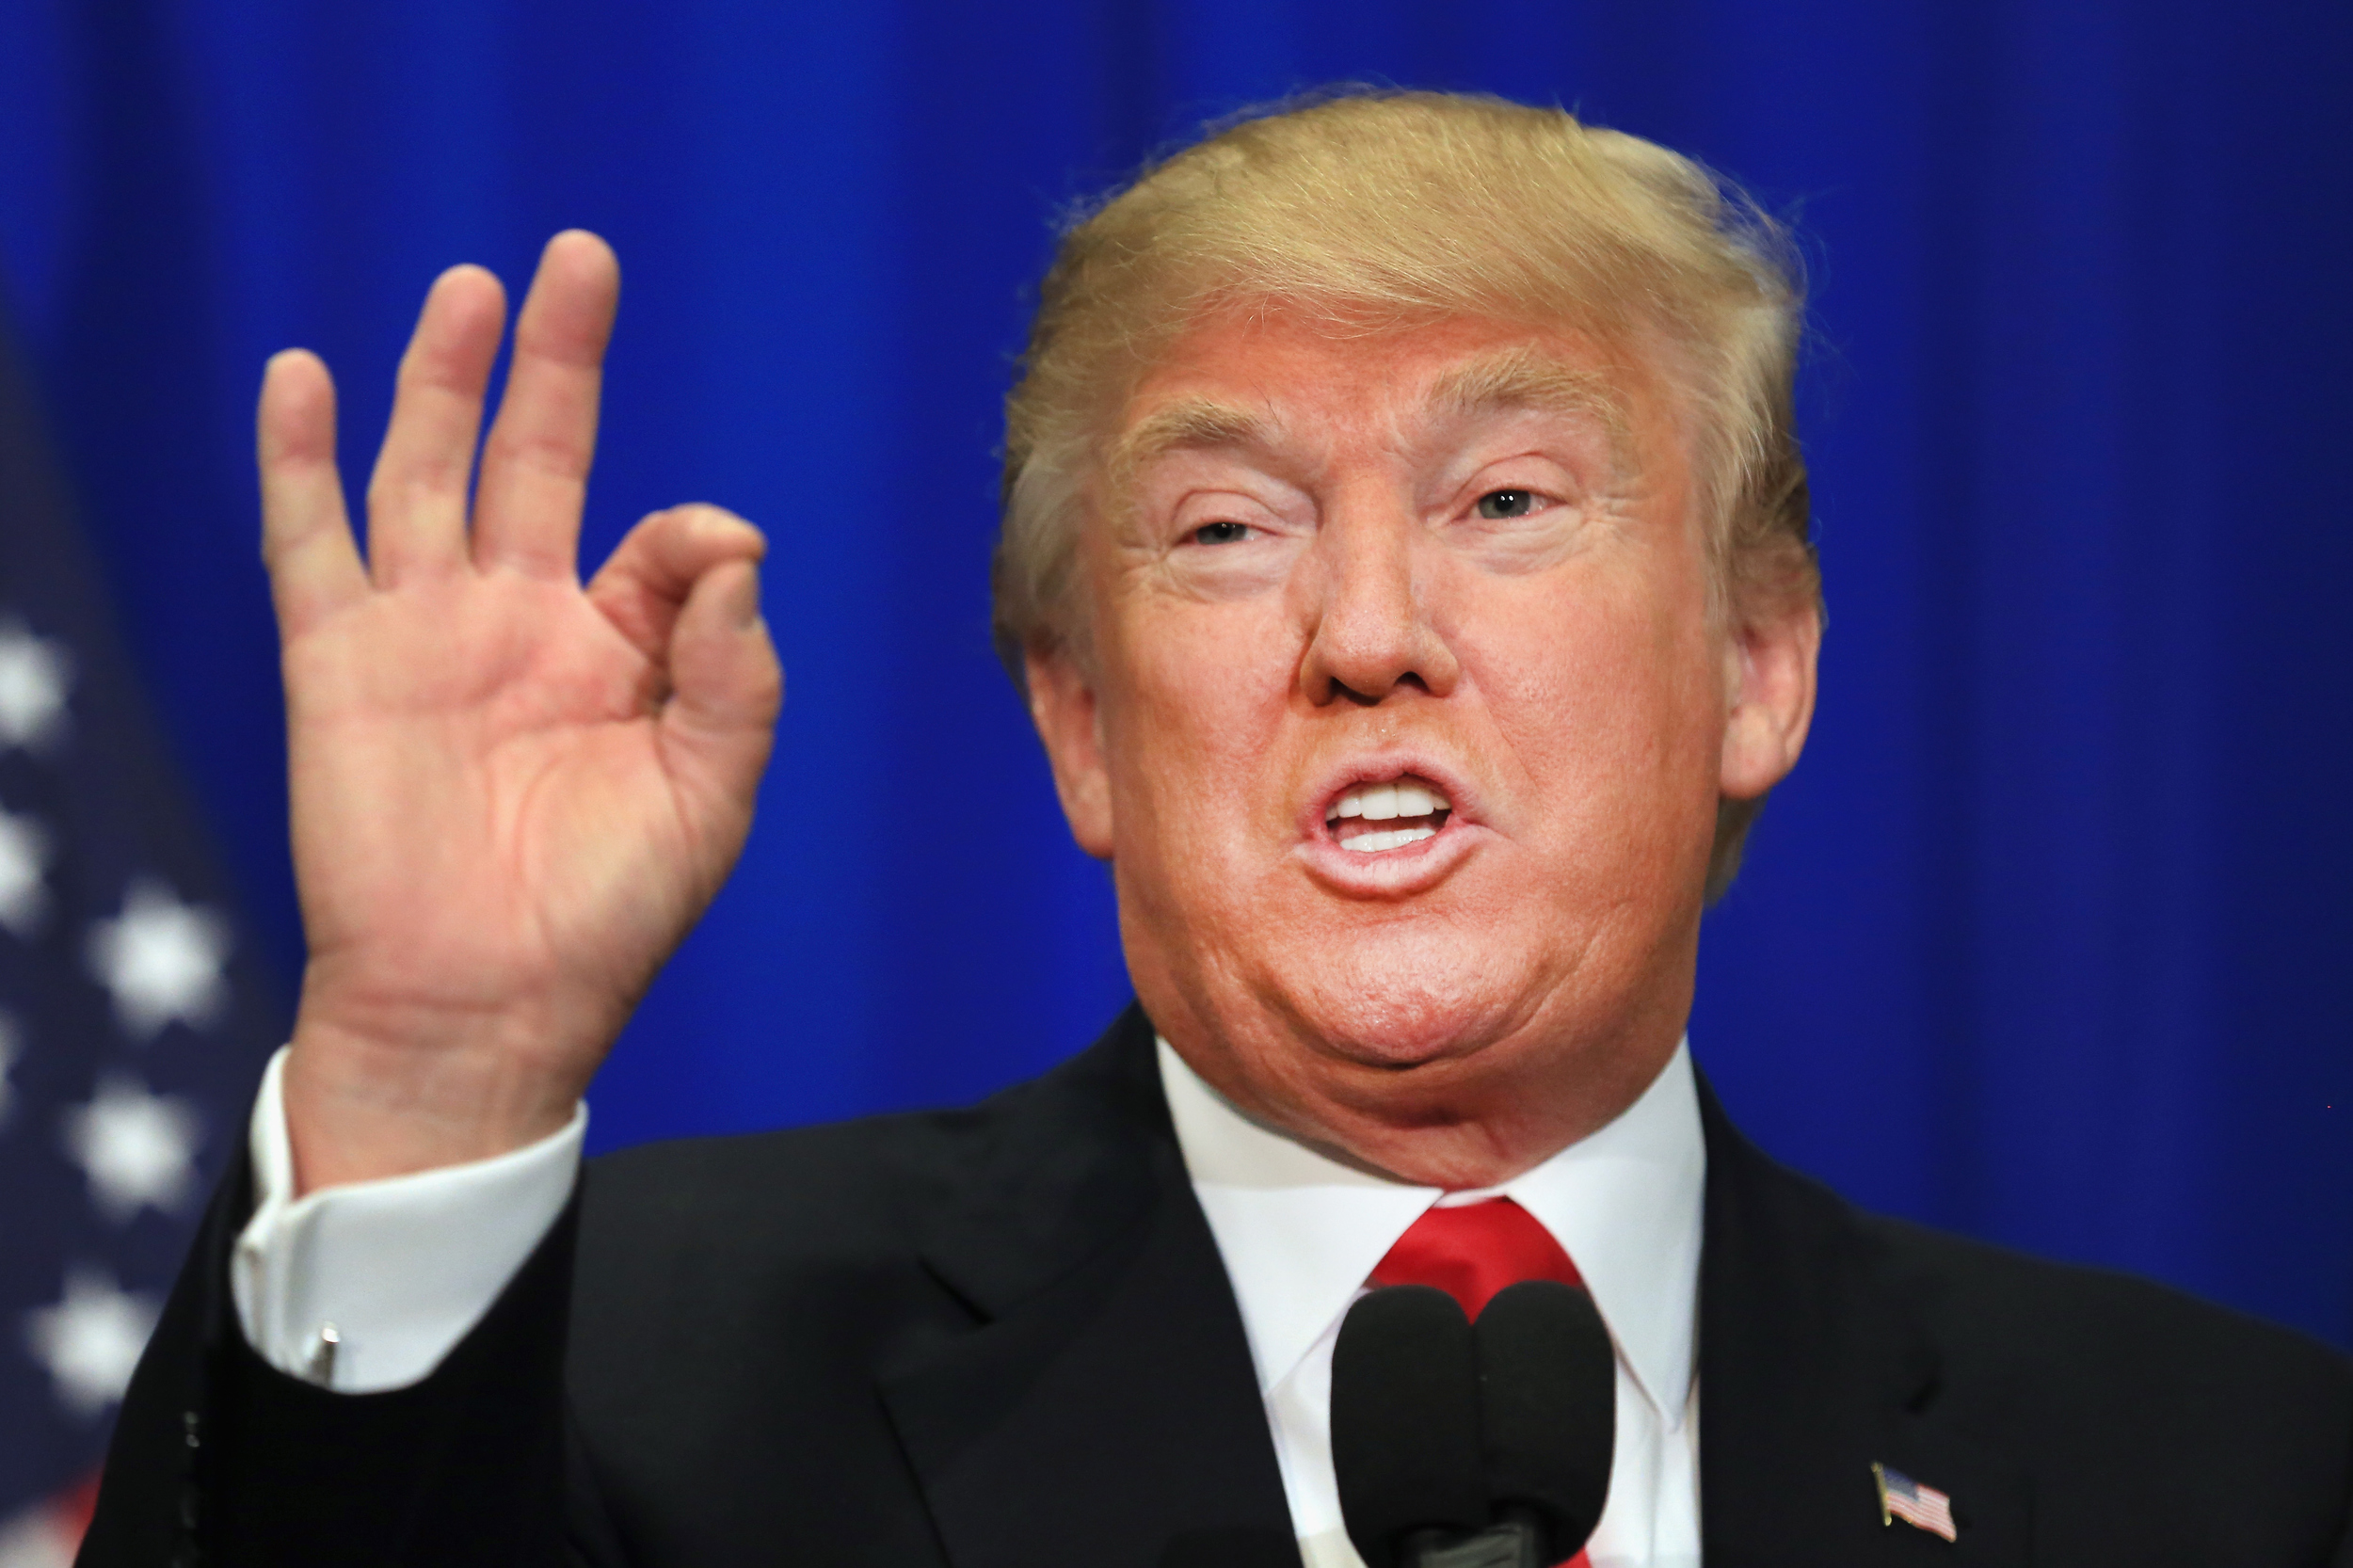
\includegraphics[width=6cm,height=4.5cm]{images/profiles/trump.jpg}
 \vskip0.5cm
 {\bfseries\Large Donald Trump}
 \begin{enumerate}[a)]
   \item Republican
   \item Bachelor's Degree in Economics from U-Penn
   \item None; he is a businessman
   \item Married and divorced, with kids
 \end{enumerate}
 &
 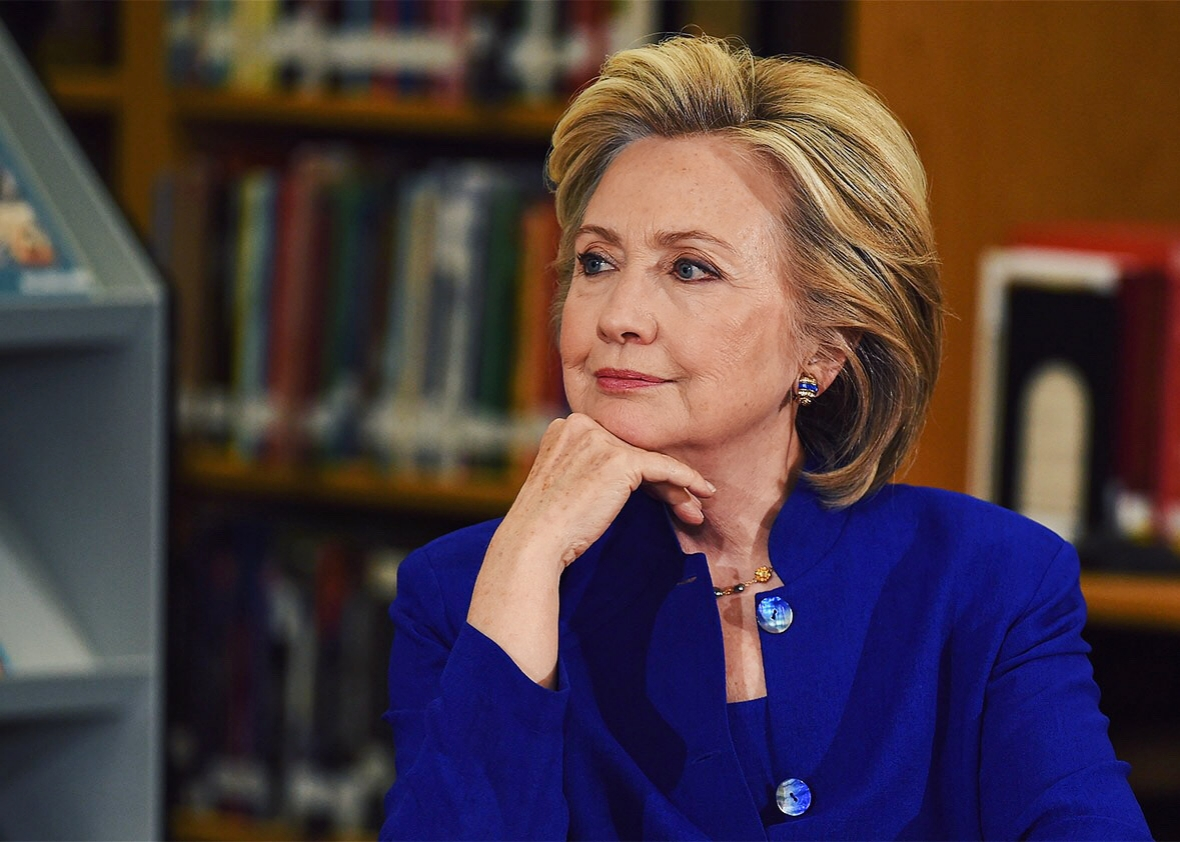
\includegraphics[width=6cm,height=4.5cm]{images/profiles/clinton.jpg}
  \vskip0.5cm
 {\bfseries\Large Hillary Clinton}
 \begin{enumerate}[a)]
   \item Democrat
   \item J.D. from Yale
   \item New York Senator, Secretary of State (not elected), First Lady
   \item Married, one daughter
 \end{enumerate}\\
\end{tabu}
\end{center}
\newpage
\section{Articles}
\subsection{September}
\subsection{October}
\subsubsection{October I}
\subsubsection{October II}
\subsection{November}
\newpage
\section{Fourier Analysis}
\vskip4cm
\paragraph{Why Fourier?} Fourier allows us to generate a function of sines and cosines to approximate another function. In this case, the function that we are approximating
is the result of the election, the expected polls. Fourier also allows us to have known turing points (points of inflection), which are to be expected day to day and correspond
with the news cycle and new things coming out about the candidates. The numbers I used are from fivethirtyeight.com. They allow you to download a .csv file with all of the polls they
analyzed and adjusted. I used the FiveThirtyEight adjusted data.

\newpage
\subsection{Clinton}
\begin{figure}[H]
  \centering
    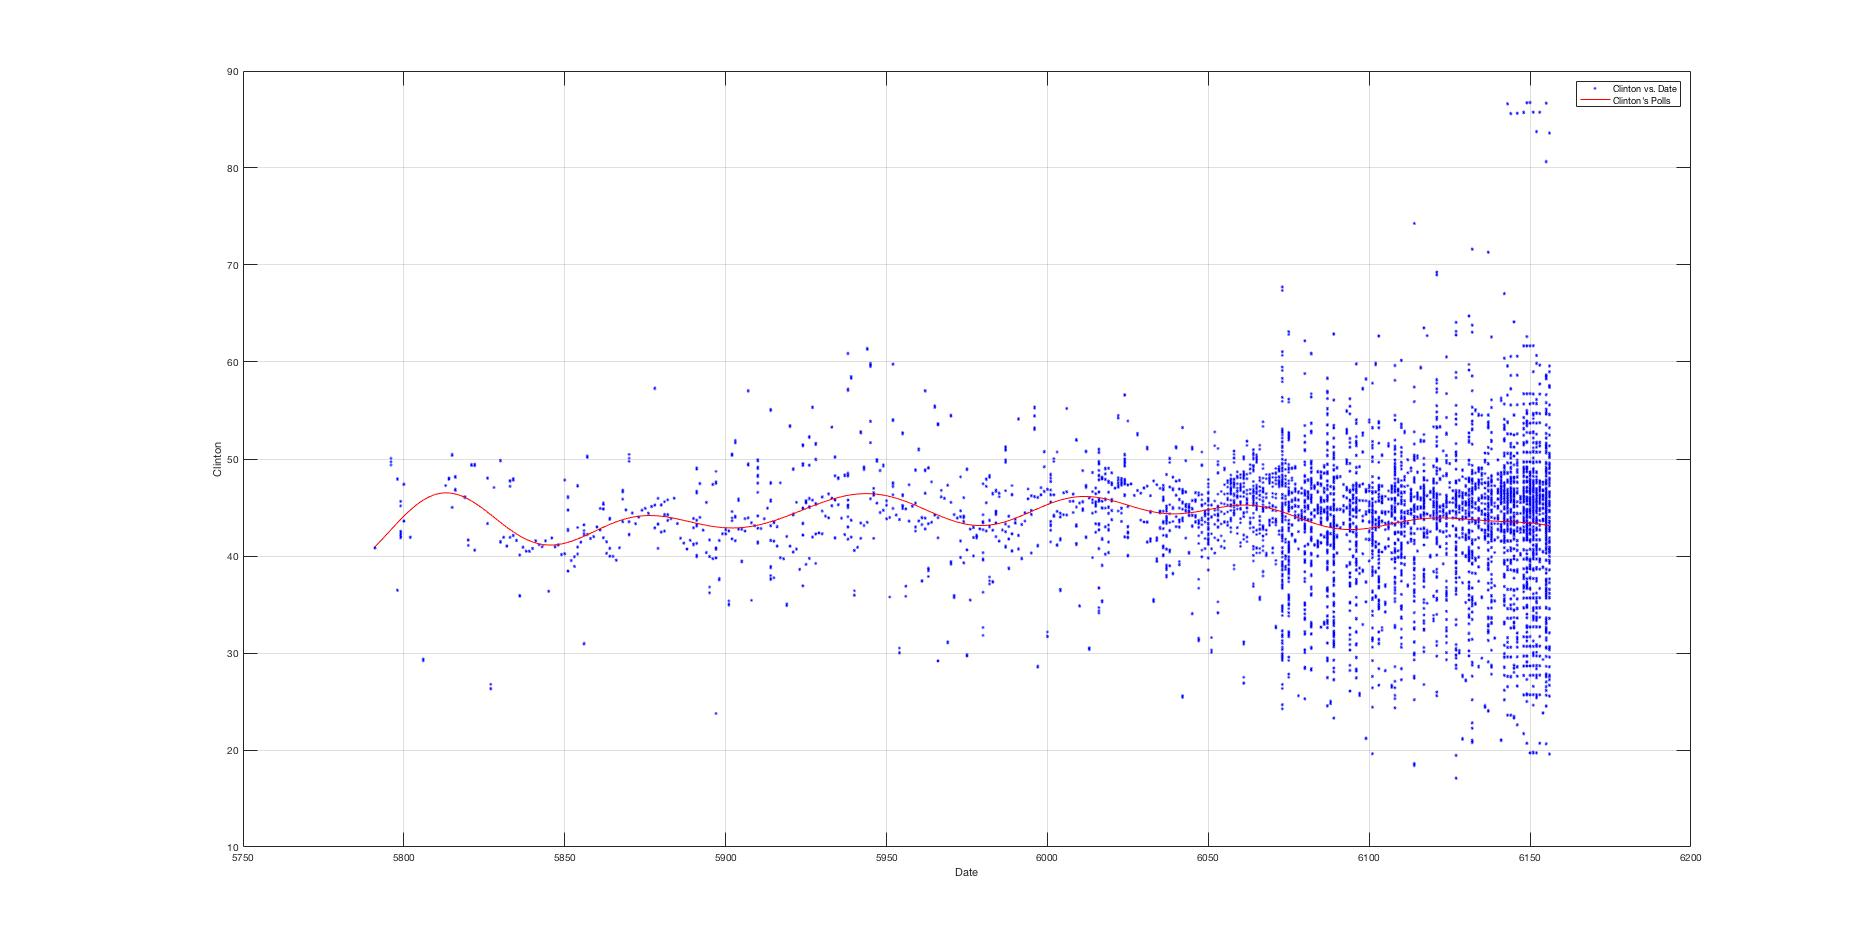
\includegraphics[width=\textwidth]{images/fourier/clinton.jpg}
    \caption{Clinton's Fourier Analysis}
\end{figure}
 \begin{figure}[H]
   \centering
     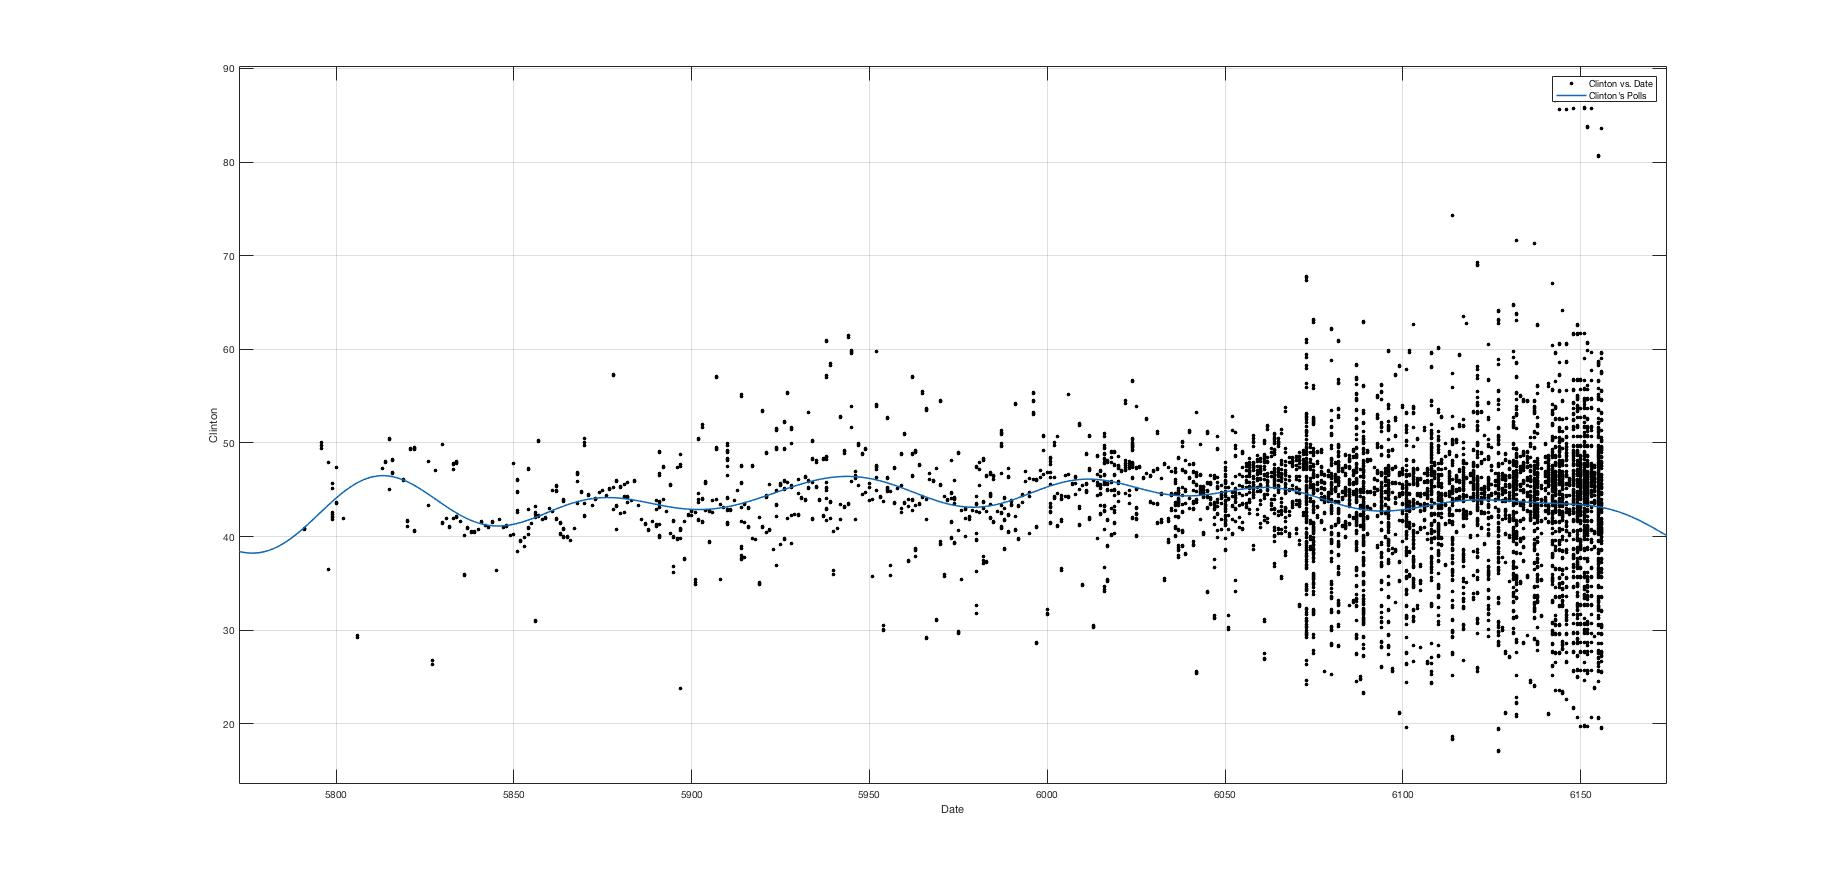
\includegraphics[width=\textwidth,height=6cm]{images/fourier/clintonlarge.jpg}
     \caption{Clintons's Fourier Extrapolation}
 \end{figure}
 \paragraph{Analysis} Clinton's Fourier analysis is very interesting. It actually shows her trending down towards the end, as was seen in the election.
  She doesn't trend below 50\%, but the trend down is very interesting to see. Her actual Fourier Analysis (of 8 terms) calculated by MATLAB with 95\% confidence is:
\newpage
\begin{gather*}
  f(x) =
           a_0 + a_1*cos(x*w) + b_1*sin(x*w) + \\
           a_2*cos(2*x*w) + b_2*sin(2*x*w) + a_3*cos(3*x*w) + b_3*sin(3*x*w) + \\
           a_4*cos(4*x*w) + b_4*sin(4*x*w) + a_5*cos(5*x*w) + b_5*sin(5*x*w) + \\
           a_6*cos(6*x*w) + b_6*sin(6*x*w) + a_7*cos(7*x*w) + b_7*sin(7*x*w) + \\
           a_8*cos(8*x*w) + b_8*sin(8*x*w)\\
\end{gather*}
Coefficients (with 95\% confidence bounds):
\begin{gather*}
   a_0 =       43.67 \\
   a_1 =       -1.41  \\
   b_1 =     -0.4745  \\
   a_2 =     -0.3162 \\
   b_2 =     0.06548  \\
   a_3 =     -0.4852  \\
   b_3 =      0.1476 \\
   a_4 =     -0.9232  \\
   b_4 =     -0.7231 \\
   a_5 =     -0.5835  \\
   b_5 =     -0.3198  \\
   a_6 =     -0.5982  \\
   b_6 =      -1.115  \\
   a_7 =      0.6509  \\
   b_7 =     -0.1644  \\
   a_8 =       0.402  \\
   b_8 =      -0.263  \\
   w =     0.01527  \\
\end{gather*}

\newpage
\subsection{Trump}
\begin{figure}[H]
  \centering
    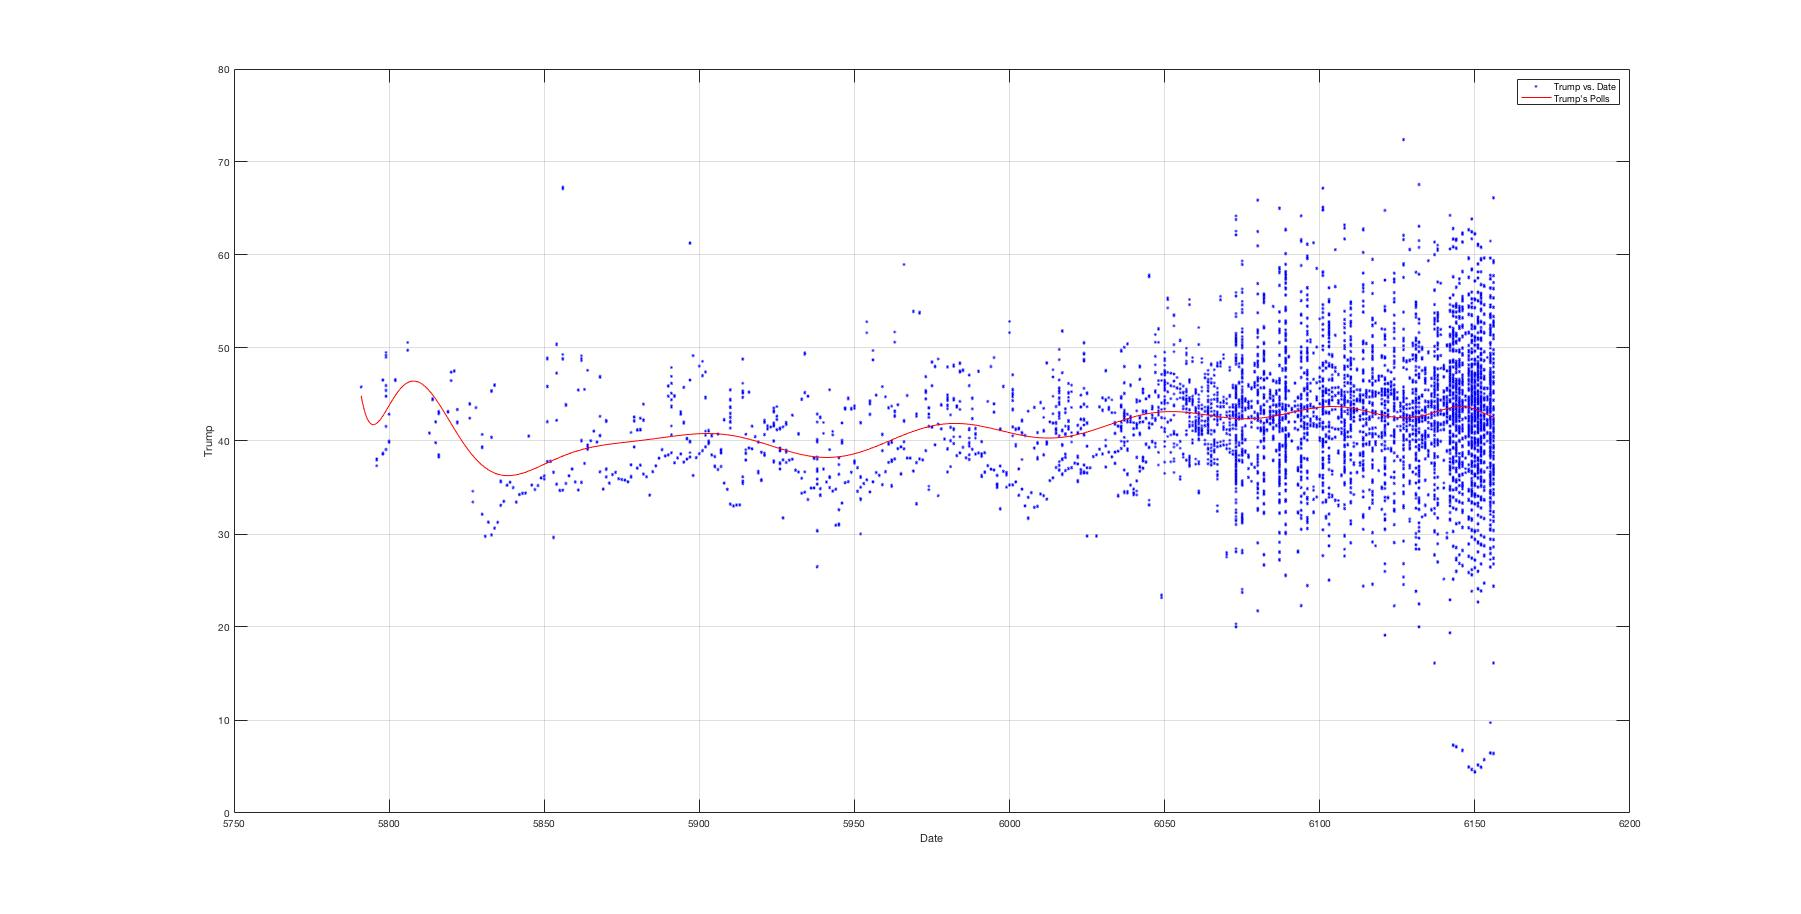
\includegraphics[width=\textwidth,height=6cm]{images/fourier/trump.jpg}
    \caption{Trump's Fourier Analysis}
\end{figure}
\begin{figure}[H]
  \centering
    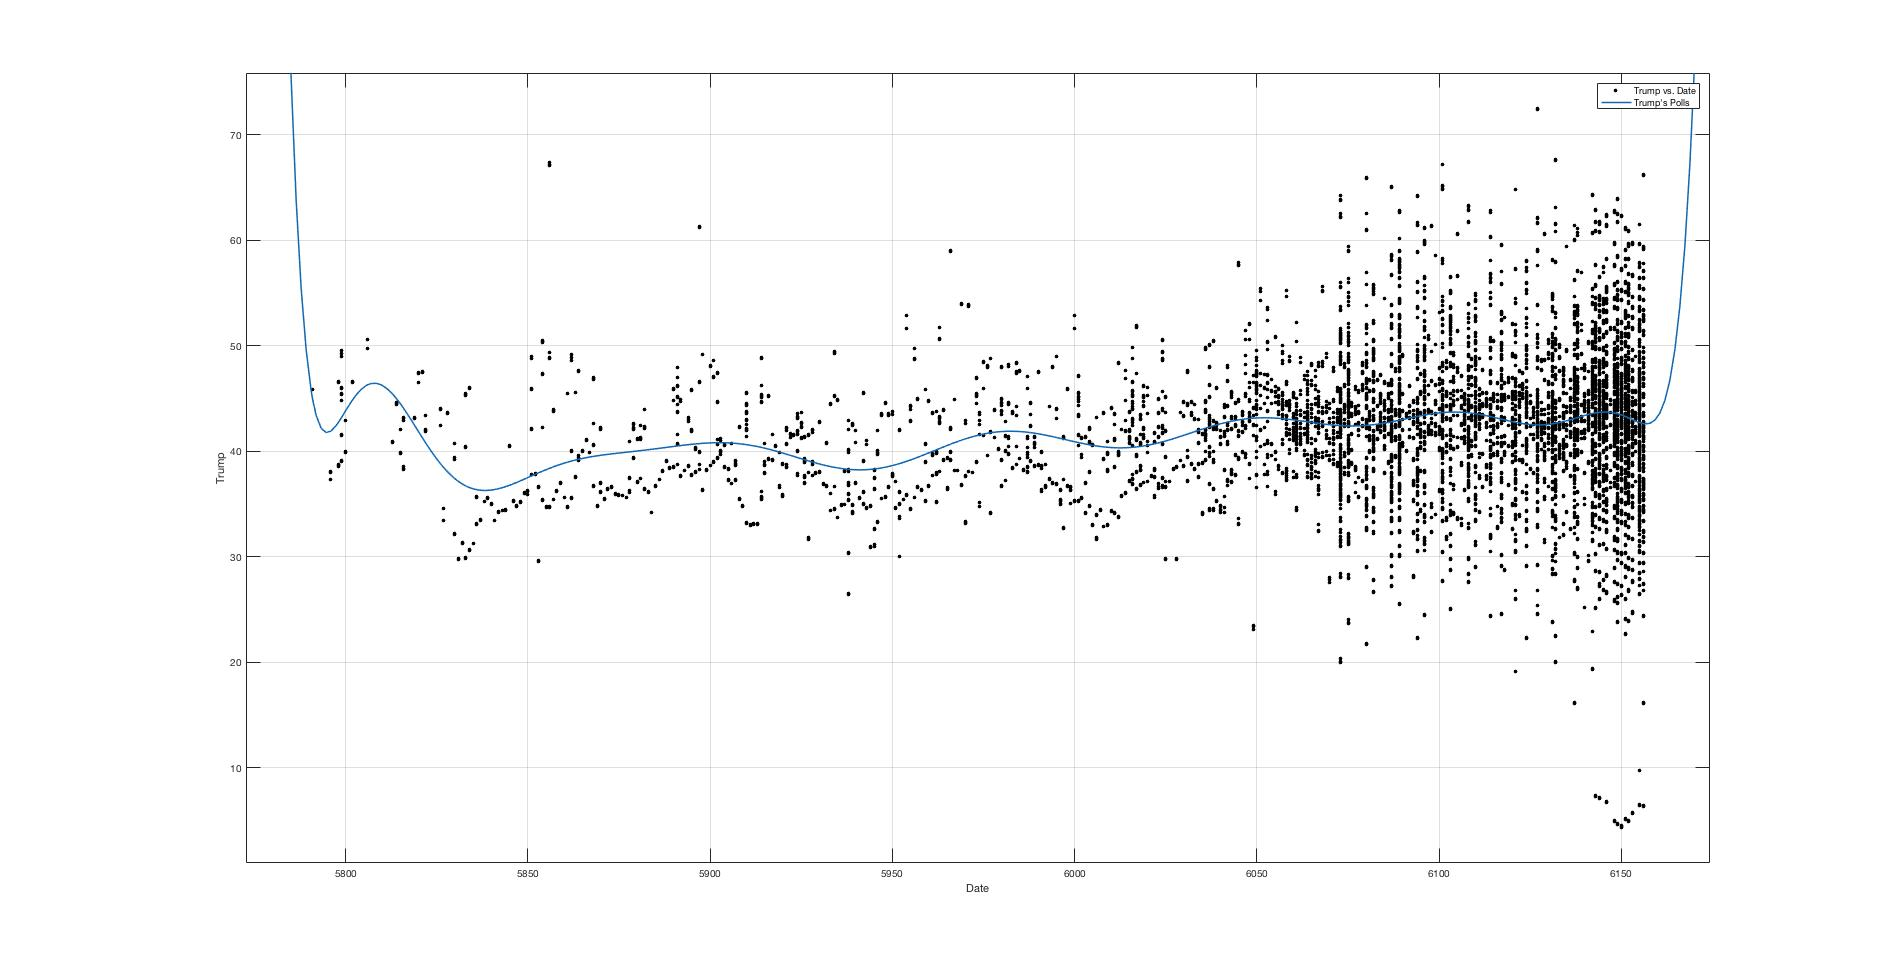
\includegraphics[width=\textwidth,height=6cm]{images/fourier/trumplarge.jpg}
    \caption{Trump's Fourier Extrapolation}
\end{figure}
\paragraph{Analysis} Trump's Fourier analysis is very interesting, too. We see the same trends as were reported by the polls, but based upon past history of Trump's numbers,
the Fourier function tells us that he will hit a point of inflection soon after November 8th. This is also apparent by the results of the election, but the point of inflection
was hit even sooner. Here's the actual analysis:
\newpage
\begin{gather*}
f(x) =
          a_0 + a_1*\cos(x*w) + b_1*\sin(x*w) +\\
          a_2*\cos(2*x*w) + b_2*\sin(2*x*w) + a_3*\cos(3*x*w) + b_3*\in(3*x*w) +\\
          a_4*\cos(4*x*w) + b_4*\sin(4*x*w) + a_5*\cos(5*x*w) + b_5*\sin(5*x*w) +\\
          a_6*\cos(6*x*w) + b_6*\sin(6*x*w) + a_7*\cos(7*x*w) + b_7*\sin(7*x*w) +\\
          a_8*\cos(8*x*w) + b_8*\sin(8*x*w)\\
\end{gather*}
Coefficients (with 95\% confidence bounds):
\begin{gather*}
  a_0 =   2.016e+06\\
  a_1 =    -1.9e+06  \\
  b_1 =   3.156e+06  \\
  a-2 =  -1.311e+06  \\
  b_2 =  -2.477e+06  \\
  a_3 =   1.756e+06  \\
  b_3 =    9.75e+04  \\
  a_4 =  -5.032e+05  \\
  b_4 =   7.383e+05  \\
  a_5 =  -1.482e+05  \\
  b_5 =  -3.238e+05  \\
  a_6 =   1.047e+05  \\
  b_6 =   1.206e+04  \\
  a_7 =  -1.273e+04  \\
  b_7 =   1.643e+04  \\
  a_8 =      -746.8  \\
  b_8 =       -1938  \\
  w =    0.007184 \\
\end{gather*}














\newpage
\section{Polls}
\section{Political Cartoons}
\section{Wisconsin State Journal Endorsements}
\subsection{President}
\subsection{Senate}
\subsection{House}
\section{My Endorsements}
\subsection{President}
\subsection{Senate}
\subsection{House}
\section{Election Results}
\section{Advice}
















\end{document}
